%new features - als
%-rotate
%-resize
%-collision
%-design changes
%	-record
%	-cam 
%	-save


\section{Key Changes}
\begin{frame}
	\frametitle{Key Changes}
	\begin{itemize}
		\item Rotation of entities
		\item Collision detection
		\item Resizing of entities
		\item Design changes
		\begin{itemize}
			\item Record dialogue
			\item Camera dialogue
			\item Save dialogue
		\end{itemize}
	\end{itemize}
\end{frame}

\begin{frame}
	\frametitle{Rotation}
	\begin{itemize}
	\item Before: Rotate Icon not click-able, but worked.
	\item After, use rotation matrix: $R = \begin{bmatrix}
			cos\, \theta & - sin\, \theta\\
			sin\, \theta & cos\, \theta
			\end{bmatrix}$
	\item Rotate point $p = \begin{bmatrix}x\\y\end{bmatrix}$ around (0,0) to get $p'$
	\item $p' = R*p$
	\item Solved rotation issue with collision detection correctly implemented for rotated entities.
	\end{itemize}
\end{frame}



\begin{frame}
	\frametitle{Collision Detection - Rectangle}
	ABP, BCP, CDP, and DAP all right turns.
		\begin{figure}
		\centering
			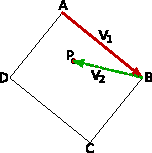
\includegraphics[width=0.6\textwidth]{media/rectangle-collision}
		\end{figure}
\end{frame}

%\begin{frame}
%	\frametitle{Collision Detection - Ellipsis}
%		\begin{figure}
%		\centering
%			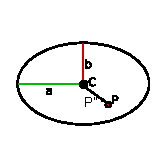
\includegraphics[width=0.6\textwidth]{media/ellipse-collision}
%		\end{figure}
%		$$\frac{ (P''_x * cos(\alpha) - P''_y * sin(\alpha))^2}{a^2} + \frac{(P''_x * sin(\alpha) - P''_y * cos(\alpha))^2}{b^2} \leq 1$$
%\end{frame}

\begin{frame}
	\frametitle{Resize}
	\begin{itemize}
		\item Old version: When resizing just add dragvector components to width and height.
		\item Was bad with large rotations
		\item New version:
		\begin{itemize}
			\item More stable
			\item Still \textit{floats} a bit, but acceptable up to $45 ^\circ$
			\item Let us utilize that when resizing!
		\end{itemize}
	\end{itemize}
\end{frame}

\begin{frame}
	\frametitle{Resize - New Version}
			\begin{figure}
			\centering
				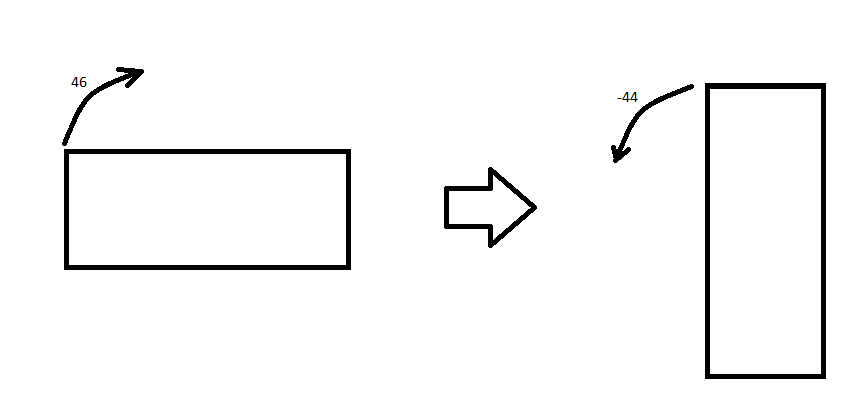
\includegraphics[width=0.6\textwidth]{approach6}
			\end{figure}
			\begin{itemize}
			\item Look at $46^\circ$ as $-44^\circ$
			\item Reset starting point of rectangle
			\item Swap width and height
			\item Then resize with dragvector
			\end{itemize}
			
\end{frame}

\begin{frame}
	\frametitle{Design Changes - Record}
	\begin{figure}
	        \centering
	        \begin{subfigure}[b]{0.24\textwidth}
	                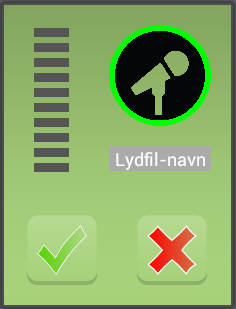
\includegraphics[width=\textwidth]{CrocOldAudio}
	        \end{subfigure}%
	        \begin{subfigure}[b]{0.24\textwidth}
	                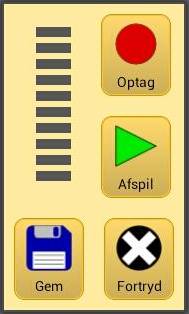
\includegraphics[width=\textwidth]{newrecordidle}
	        \end{subfigure}
	        \begin{subfigure}[b]{0.24\textwidth}
	                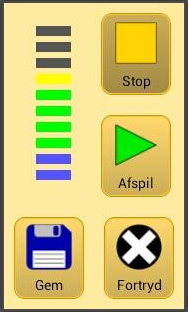
\includegraphics[width=\textwidth]{newrecording}
	        \end{subfigure}
 	        \begin{subfigure}[b]{0.24\textwidth}
 	                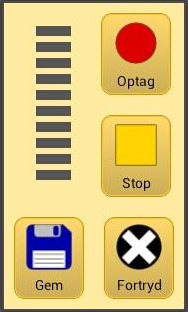
\includegraphics[width=\textwidth]{newrecordplay}
 	        \end{subfigure}
	\end{figure}
\end{frame}

%flere slides til design changes
\begin{frame}
	\frametitle{Design Changes - Camera, Old}
	Switch to camera.
		\begin{figure}
		\centering
			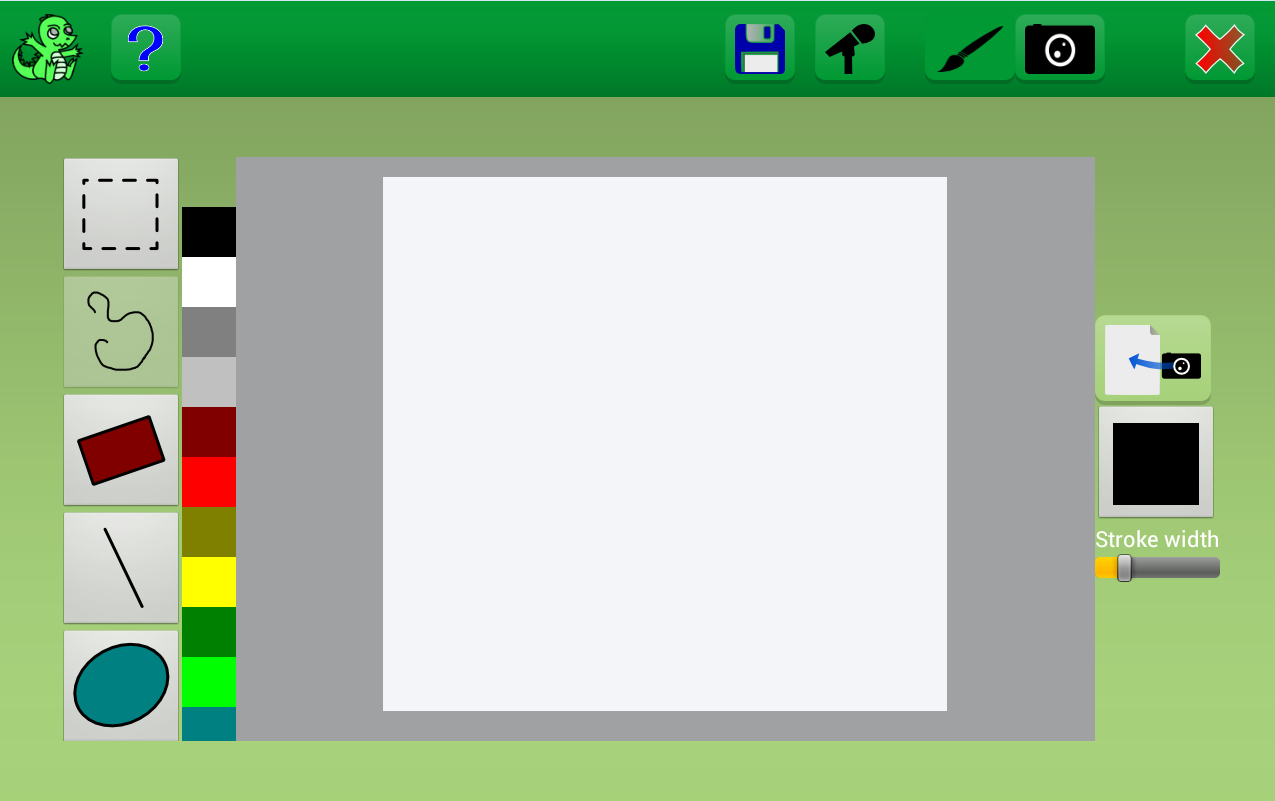
\includegraphics[width=0.8\textwidth]{CrocOldCanvas}
		\end{figure}
\end{frame}

\begin{frame}
	\frametitle{Design Changes - Camera, Old}
	Take picture.
		\begin{figure}
		\centering
			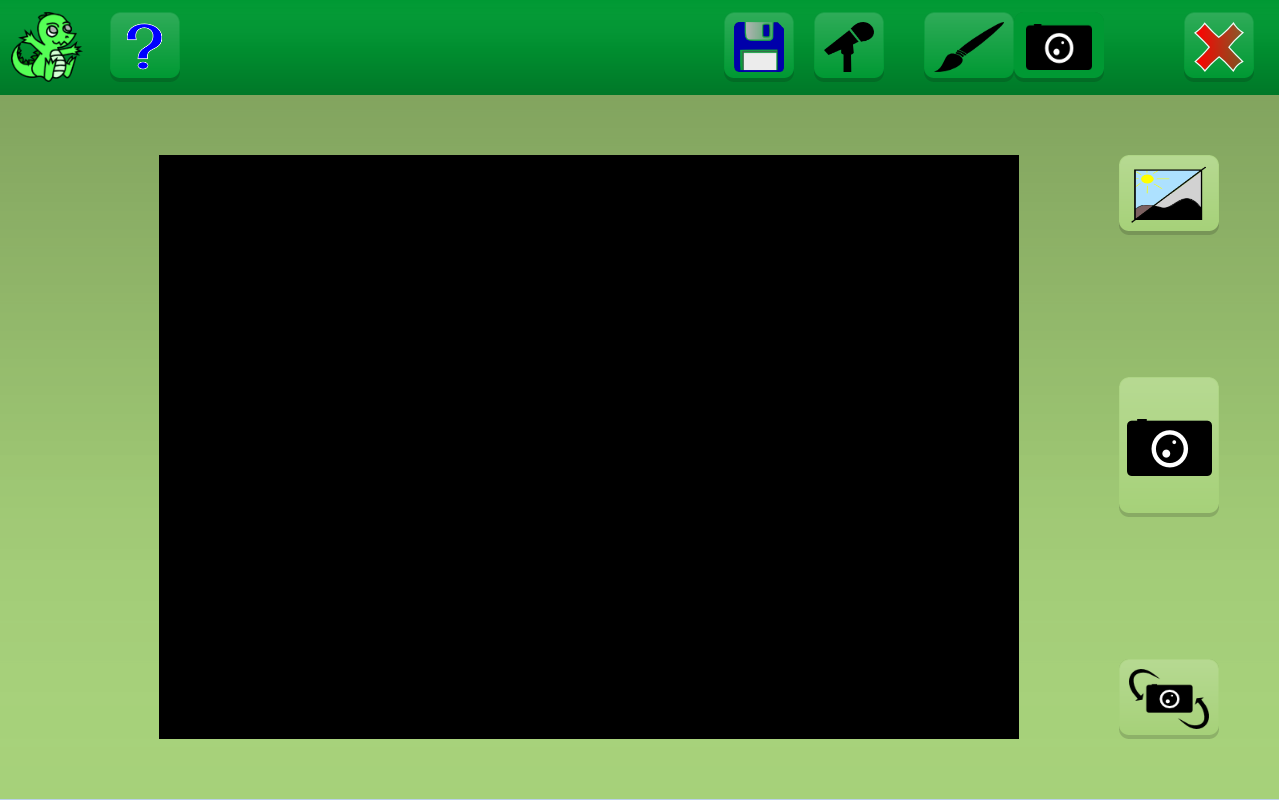
\includegraphics[width=0.8\textwidth]{CrocOldCamera}
		\end{figure}
\end{frame}

\begin{frame}
	\frametitle{Design Changes - Camera, Old}
	Load picture.
		\begin{figure}
		\centering
			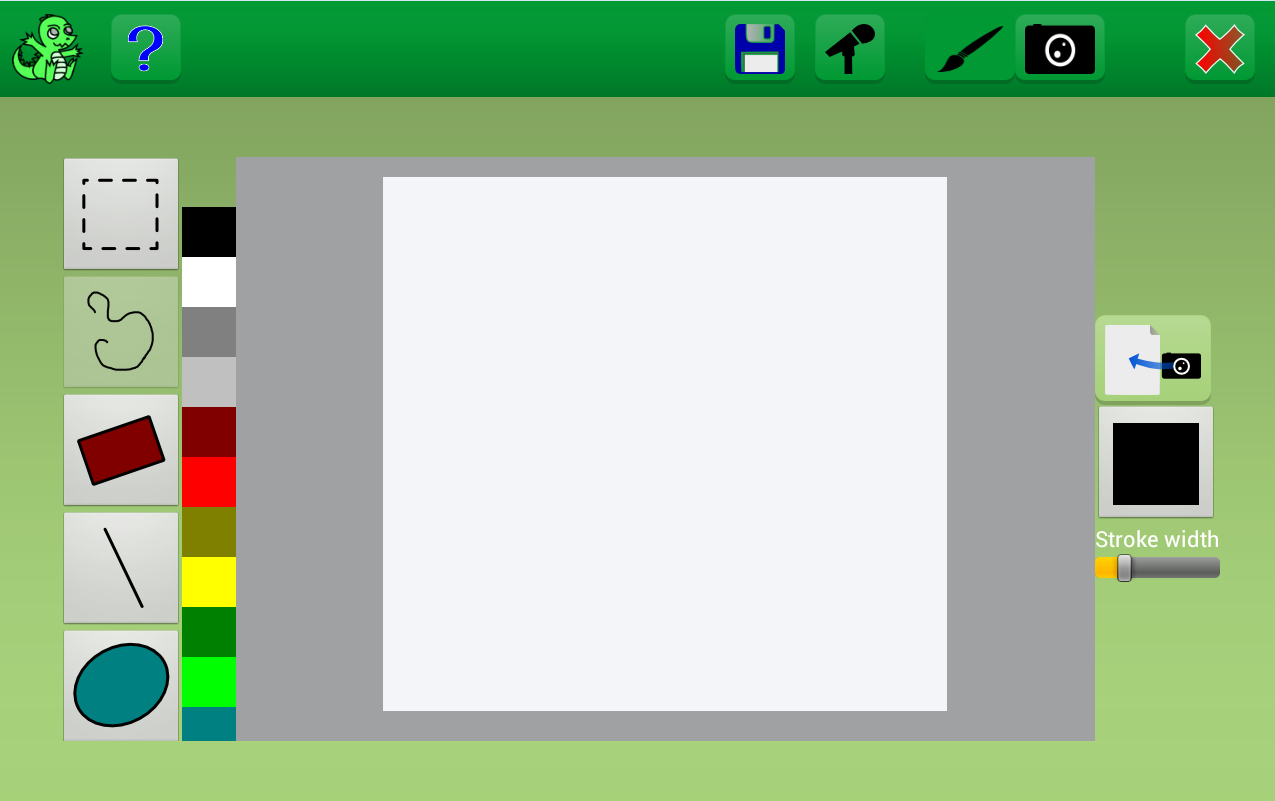
\includegraphics[width=0.8\textwidth]{CrocOldCanvas}
		\end{figure}
\end{frame}

\begin{frame}
	\frametitle{Design Changes - Camera, Old}
	Load picture.
		\begin{figure}
		\centering
			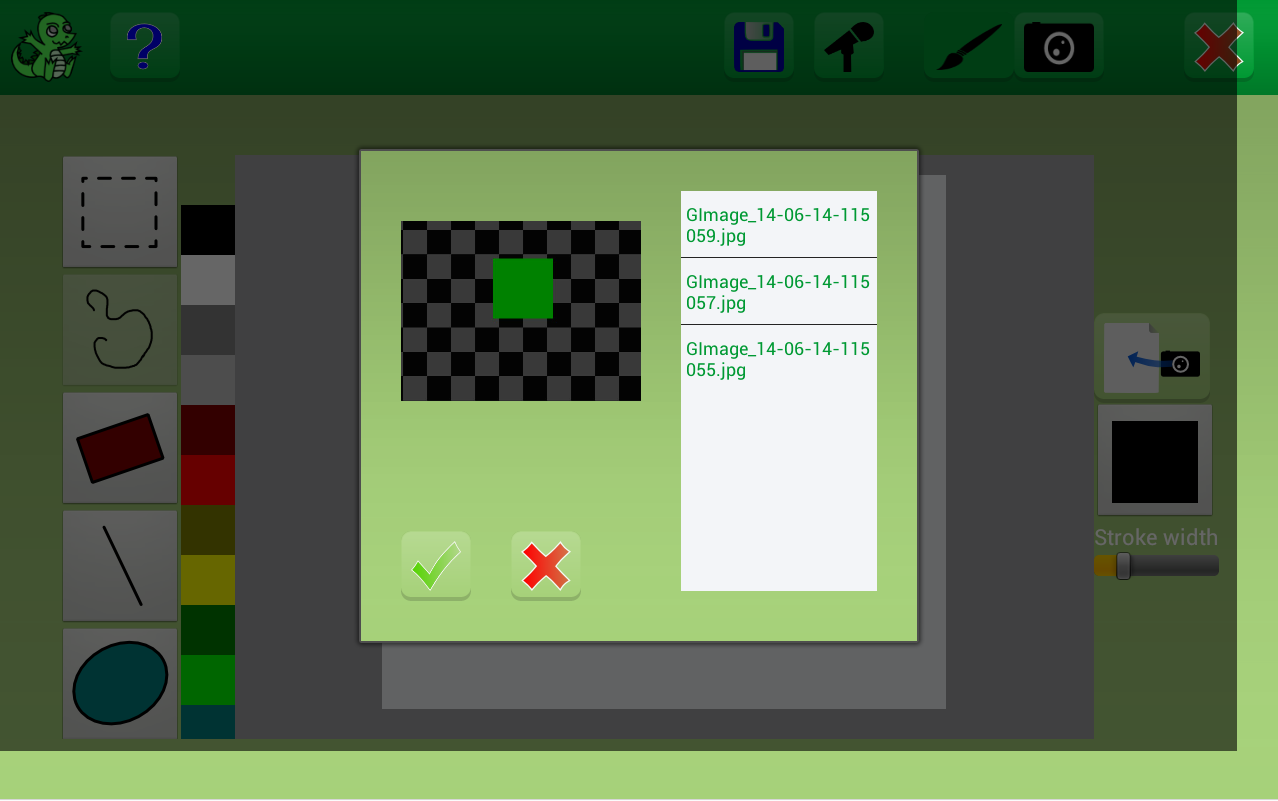
\includegraphics[width=0.8\textwidth]{cameraload}
		\end{figure}
\end{frame}
%flere slides til design changes
\begin{frame}
	\frametitle{Design Changes - Camera}
	\begin{itemize}
		\item Old way was deemed unintuitive
		\item Customers wanted a way to take pictures similar to other camera apps
		\item Inspiration from Instagram and iOS camera app
	\end{itemize}
\end{frame}

\begin{frame}
	\frametitle{Design Changes - Camera, New}
	Open camera
		\begin{figure}
		\centering
			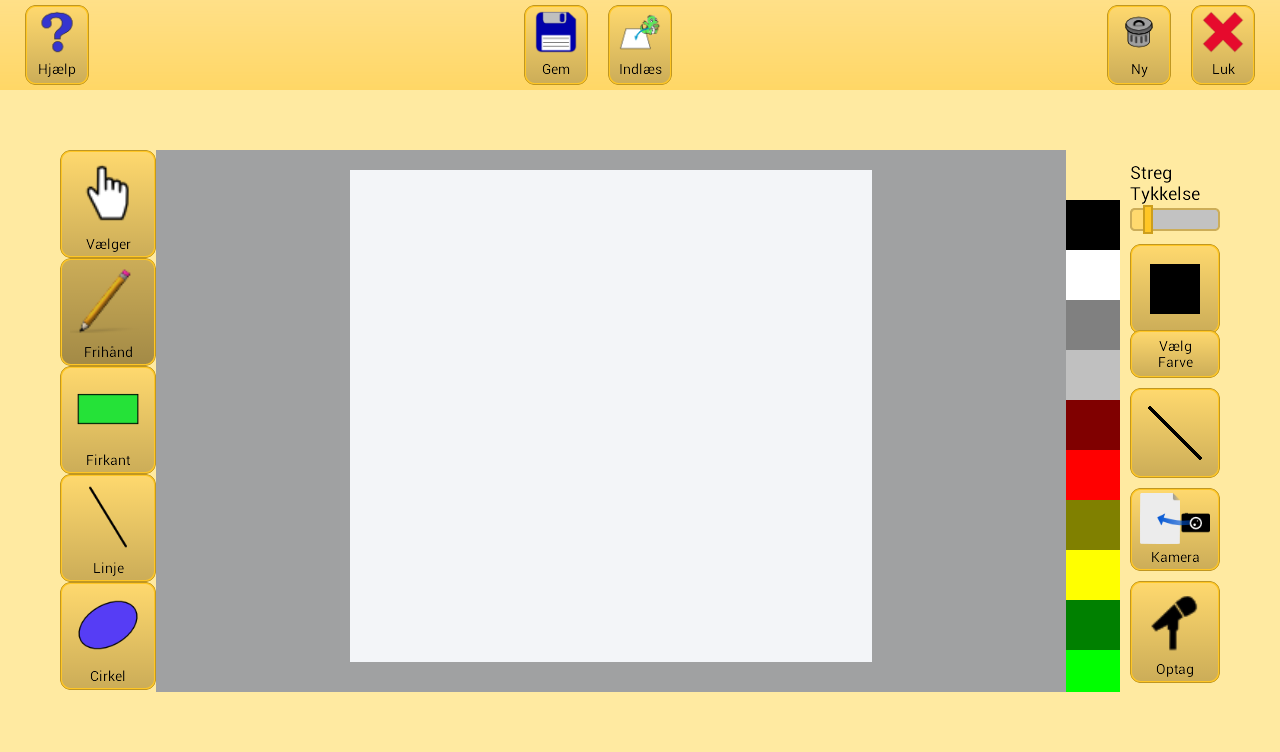
\includegraphics[width=0.8\textwidth]{final-main-ui}
		\end{figure}
\end{frame}

\begin{frame}
	\frametitle{Design Changes - Camera, New}
	Take picture
		\begin{figure}
		\centering
			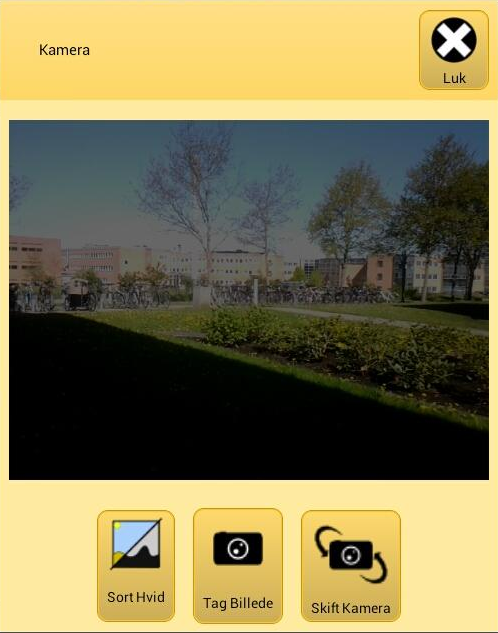
\includegraphics[width=0.5\textwidth]{cam1}
		\end{figure}
\end{frame}

\begin{frame}
	\frametitle{Design Changes - Camera, New}
	Accept picture
		\begin{figure}
		\centering
			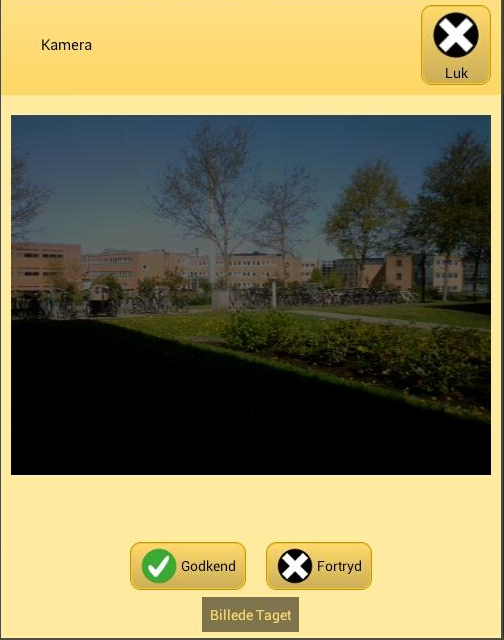
\includegraphics[width=0.5\textwidth]{cam2}
		\end{figure}
\end{frame}

\begin{frame}
	\frametitle{Design Changes - Camera, New}
	Result
		\begin{figure}
		\centering
			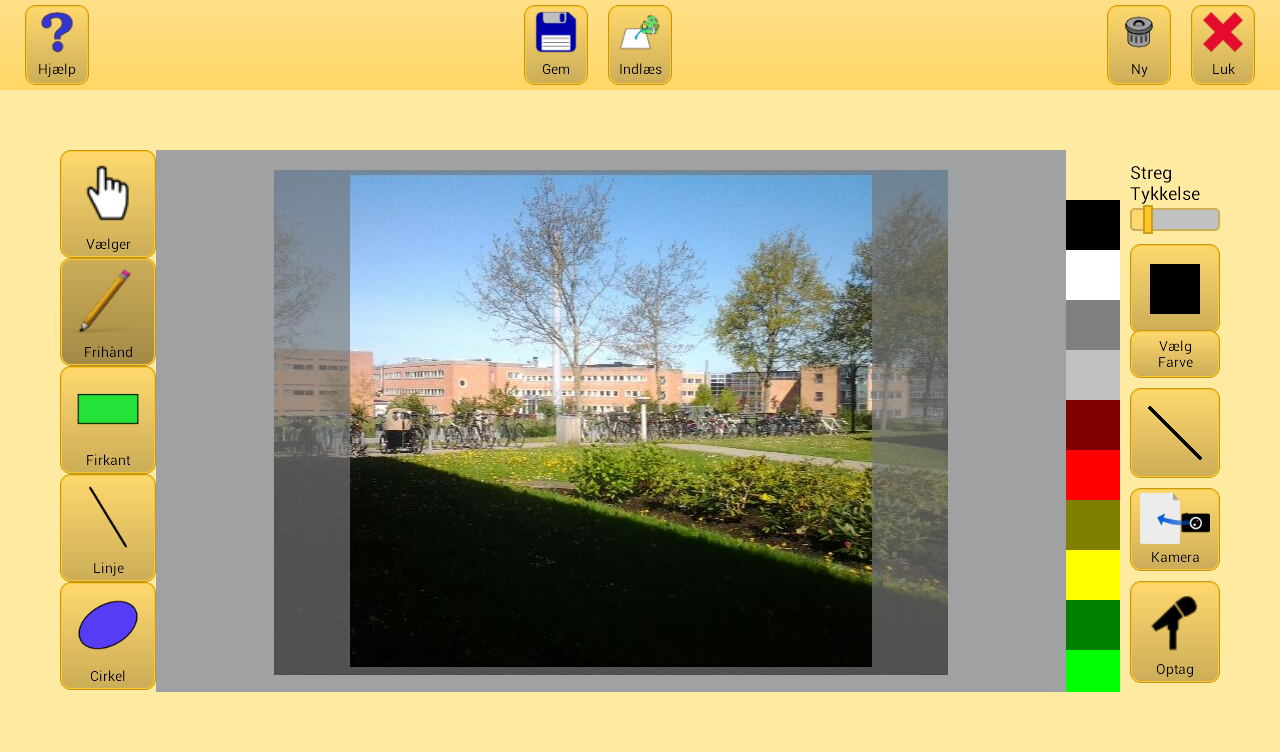
\includegraphics[width=0.8\textwidth]{cam3}
		\end{figure}
\end{frame}
%flere slides til design changes
\begin{frame}
	\frametitle{Design Changes - Save Dialogue}
	\begin{itemize}
	\item Database not finished previous years
	\item A dialogue was made, but functionality to save was not.
	\item Now able to save pictograms as the database got developed.
	\end{itemize}
\end{frame}

\begin{frame}
	\frametitle{Design Changes - Save, Old}
		\begin{figure}
		\centering
			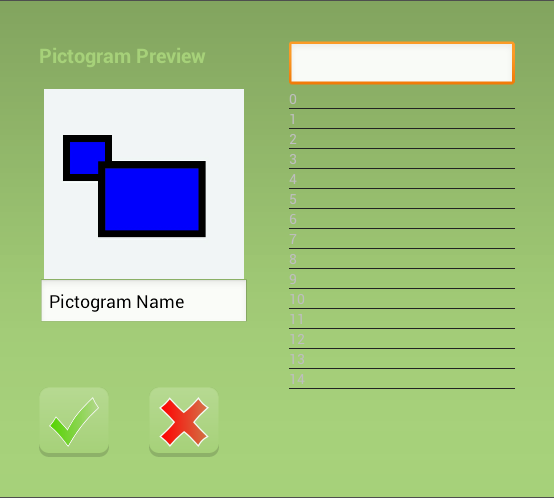
\includegraphics[width=0.8\textwidth]{saveold}
		\end{figure}
\end{frame}

\begin{frame}
	\frametitle{Design Changes - Save, New}
		\begin{figure}
		\centering
			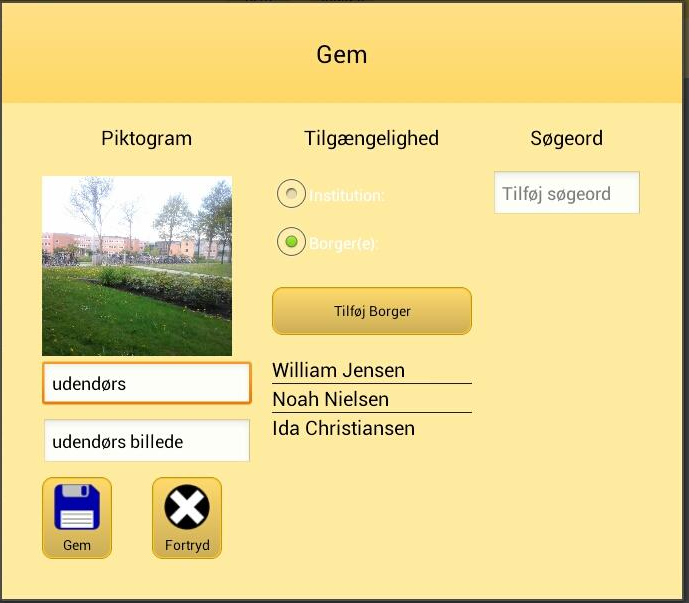
\includegraphics[width=0.8\textwidth]{savenew}
		\end{figure}
\end{frame}